\documentclass{beamer}
\usetheme{metropolis}
\usepackage{graphicx}
\usepackage{amsmath}
\usepackage{tcolorbox}
\title{College Writing Seminar (INTD100): Week 5 Notes}
\author{Jordan Hanson}
\institute{Whittier College Department of Physics and Astronomy}

\begin{document}
\maketitle

\section{Summary}

\begin{frame}{Summary}
\small
\textbf{Week 5}: \textit{The Laboratory Report I:} We will learn the major components of lab reports.  Abstracts, sections and subsections, figures, tables, captions, and how to make them flow and keep the thread of logic intact.
\begin{enumerate}
\item Exercises: how to include a graphic, figure, or table into your writing, and write about it correctly
\item Exercises: how to write an abstract correctly
\item Exercises: how to organize a report into sections and sub-sections
\item Homework: use the map technique to create sections and subsections
\item Homework: trade tracts of writing with someone, and see if they can understand your passive voice style
\end{enumerate}
\end{frame}

\section{Review of Passive Voice}

\begin{frame}{Review of Passive Voice}
Identify the subject, verb, and object in the following:
\begin{itemize}
\item We edited the genome of the fly to produce the albino color in the offspring.
\item We lured a large female hammerhead shark with bait, and then tagged her with a GPS unit.
\item Researchers piloted the drone out over the ocean, looking for signs of the whale pod.
\end{itemize}
Now cut the subject word, and reverse the order of the object and verb.  Finally, re-conjugate the verb.
\end{frame}

\begin{frame}{Review of Passive Voice}
\textit{\alert{Work in paris to convert to passive voice.}} \\
This review article outlines the key concepts in vaccine epidemiology, such as basic reproductive numbers, force of infection, vaccine efficacy and effectiveness, vaccine failure, herd immunity, herd effect, epidemiological shift, disease modeling.  This review also describes the application of this knowledge both at program levels and in the practice by family physicians, epidemiologists, and pediatricians. We make the case for increased knowledge and understanding of vaccine epidemiology among key stakeholders including policy makers, immunization program managers, public health experts, pediatricians, family physicians, and others involved in immunization service delivery.
\end{frame}

\section{Writing about a DIY Experiment}

\begin{frame}{Writing about a DIY Experiment}
\small
\textbf{\alert{You are in your house anyways, so why not experiment?}} Write down the process for completing an experiment in your house.  Examples are listed below.  Research how to accomplish your chosen project.  Write down a cohesive set of instructions in passive voice with technically accurate language.  \textbf{Exchange documents with a partner and attempt to perform the procedure they outline.}
\begin{enumerate}
\item Create a compass with a needle, magnetizing magnet, cork, and bowl of water
\item Measure the acceleration of gravity from the period of a pendulum
\item Create a ``homopolar'' motor with a copper wire and a magnet
\item Create a lemon battery
\item Measure the acceleration of gravity by timing the fall of an object
\end{enumerate}
\end{frame}

\section{Components of a Laboratory Report}

\begin{frame}{Components of a Laboratory Report}
Components of a scientific result:
\begin{itemize}
\item \textbf{Abstract}: a short pararaph near the title summarizing the work, and leaving the reader convinced the work was interesting, relevant, and with the key results.
\item \textbf{Sections and sub-sections}: if the writer has mapped or outlined the paper ahead of time, the sections and sub-sections should follow the map
\begin{itemize}
\item Introduction
\item Setup/methods
\item Data collection and analysis
\item Conclusion
\end{itemize}
\item \textbf{Figures and Tables}: graphical and analytical objects accompanied by captions that help the reader understand the results.
\end{itemize}
\end{frame}

\section{Components of a Laboratory Report: the Abstract}

\begin{frame}{Writing Abstracts}
\small
\textbf{Abstract}: a short pararaph near the title summarizing the work, and leaving the reader convinced the work was interesting, relevant, and with the key results.  Use the following information to create an abstract:
\begin{enumerate}
\item The frequency of a pendulum squared times the pendulum length is proportional to the Earth's gravitational acceleration.
\item A pendulum was created from a golf ball, and a fishing line with length 75 cm.
\item The number of times the pendulum swung back to the same place in 1 minute was measured.
\item The frequency is the number of times divided by one minute.
\item The frequency squared times $(2\pi)^2$ times the length is equal to $g$, the acceleration due to gravity of the Earth.
\item The idea that $g$ is proportional to the frequency squared is derived from Newton's Laws.
\end{enumerate}
\end{frame}

\begin{frame}{Writing Abstracts}
\small
\textbf{Result:} \\
According to Newton's Laws, the gravitational acceleration of the Earth $g$ should be weaker farther from sea level.  The value of $g$ can be derived from the frequency of a pendulum.  A pendulum was constructed using $L = 75$ cm of fishing line, tied to a golf ball.  The pendulum was perturbed and allowed to swing for $\Delta t = 1$ minute.  The number of times $N$ that the pendulum returned to the original position was recorded.  The frequency of the pendulum is $f = N/\Delta t$.  Using Newton's 2nd law, it may be shown that $g = (4\pi)^2 f^2 L$.  A result of $g = 9.8$ m/s$^2$ was obtained at sea level.  The value of $g$ was measured also on top of a 10,000 ft. mountain.  The results were found to be identical to three significant digits.
\end{frame}

\begin{frame}{Writing Abstracts}
\small
\textbf{Try it yourself:}
\begin{enumerate}
\item A survey was sent to Whittier College business administration department graduates.
\item The number of Whittier College graduates who graduated with degrees in business administration from 2010-2020 was obtained from the Registrar, along with names and contact information.
\item The survey contained the question "Indicate which of the following caused you to choose your major: (a) potential financial impact in my first career role after college (b) I wanted to start my own business (c) I wanted to understand how business works in order to improve an existing company."
\item Thirty-nine percent of survey respondents chose (a), 42 respondents chose (b), and 19 percent chose (c).
\item The number of responses to the survey was 200.
\end{enumerate}
\end{frame}

\begin{frame}{Writing Abstracts}
Polishing abstracts:
\begin{enumerate}
\item Concise writing rules are especially important, because the abstract must be \textit{short}
\item Arrange ideas from ``big to small,'' most general to the most detailed
\item Purpose \textit{of the beginning of} the abstract: convince the reader its interesting
\item Purpose \textit{of the end of} the abstract: show the reader the results
\item Include in the absract anything that is being done for the first time, or improving upon something done before
\item The abstract is the one component of a lab report or article in which the writer may use hyperbole, and it's still shaky
\end{enumerate}
\end{frame}

\begin{frame}{Writing Abstracts}
\small
\textbf{Result:} \\
\textbf{\alert{According to Newton's Laws, the gravitational acceleration of the Earth $g$ should be weaker farther from sea level.}}  \textit{The value of $g$ can be derived from the frequency of a pendulum.}  A pendulum was constructed using $L = 75$ cm of fishing line, tied to a golf ball.  The pendulum was perturbed and allowed to swing for $\Delta t = 1$ minute.  The number of times $N$ that the pendulum returned to the original position was recorded.  The frequency of the pendulum is $f = N/\Delta t$.  Using Newton's 2nd law, it may be shown that $g = (4\pi)^2 f^2 L$.  \alert{A result of $g = 9.8$ m/s$^2$ was obtained at sea level.  The value of $g$ was measured also on top of a 10,000 ft. mountain.}  \textbf{\alert{The results were found to be identical to three significant digits.}} Although being atop the mountain makes the pendulum farther from the Earth's core, and therefore the gravity weaker, the gravity of the mountain itself can be shown to compensate.
\end{frame}

\section{Components of a Laboratory Report: Sections and Subsections}

\begin{frame}{Creating Sections and Sub-Sections}
\textbf{Sections and sub-sections}: if the writer has mapped or outlined the paper ahead of time, the sections and sub-sections should follow the map
\begin{figure}
\centering
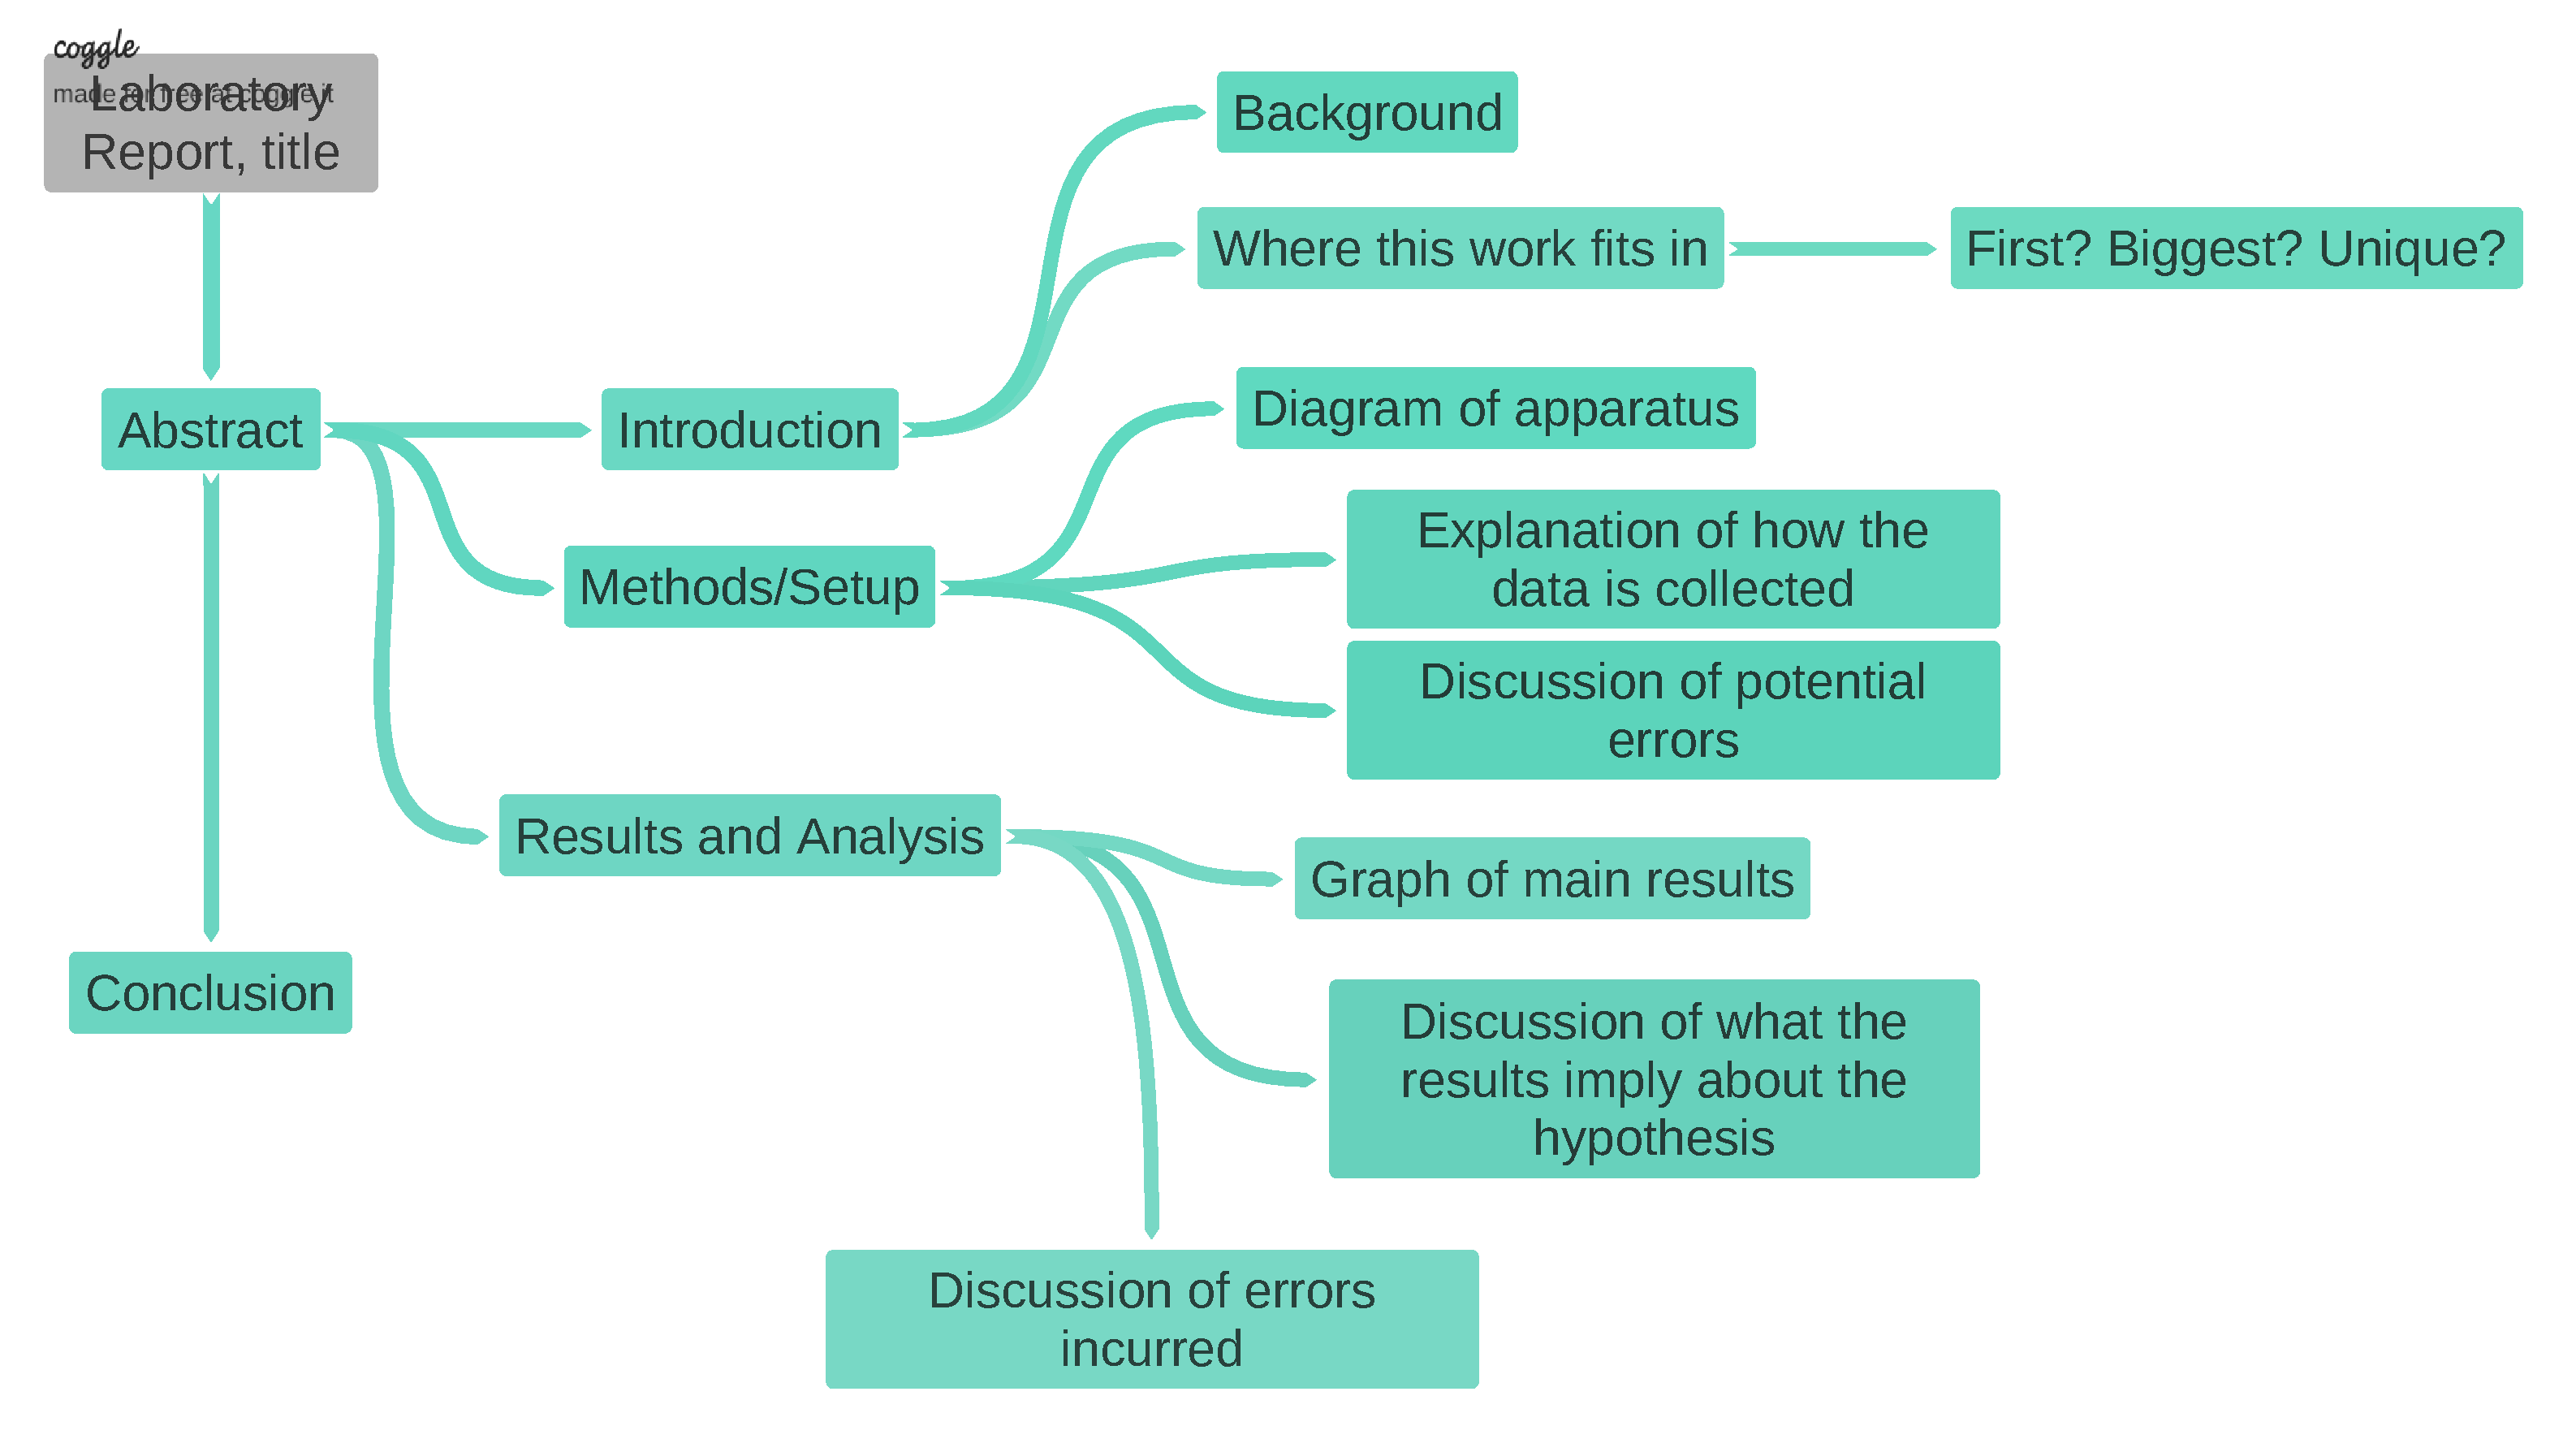
\includegraphics[width=0.75\textwidth]{figures/map1.pdf}
\caption{\label{fig:maplab} An example of how a lab report or article could be organized.}
\end{figure}
\end{frame}

\begin{frame}{Creating Sections and Sub-Sections}
Recall the summary report about vaccines.  Determine in which \textit{section} the following passages belong. \\ \vspace{0.25cm}
In modern times, John Snow (1813‑1858) and William Farr (1807‑1883) pioneered the work on epidemiology and are often referred as one of the ``fathers of modern epidemiology.'' [7,8] Epidemiology, though practiced from earlier times than vaccinology, gained attention and prominence in the 19th century. Now, the practice of vaccinology has become closely linked with that of epidemiology.
\begin{itemize}
\item Intro/Historical background
\item Vaccine Epidemiology
\item Other Important Concepts in Epidemiology
\item Conclusion
\end{itemize}
\end{frame}

\begin{frame}{Creating Sections and Sub-Sections}
Recall the summary report about vaccines.  Determine in which \textit{section} the following passages belong. \\ \vspace{0.25cm} The understanding of vaccine epidemiology has potential to save additional lives from vaccine preventable diseases and improve health outcomes through life course. The vaccine epidemiology has definitive role in extending the benefits of vaccines to additional populations and in the selection of target groups for vaccination.
\begin{itemize}
\item Intro/Historical background
\item Vaccine Epidemiology
\item Other Important Concepts in Epidemiology
\item Conclusion
\end{itemize}
\end{frame}

\begin{frame}{Creating Sections and Sub-Sections}
Recall the summary report about vaccines.  Determine in which \textit{section} the following passages belong. \\ \vspace{0.25cm}
Herd immunity may be defined as the resistance of a group or a community in total, against the invasion and spread of an infectious agent as a result of a large proportion of individuals in the group being immunized. Herd immunity or contact immunity develops in the case of certain live vaccines(e.g.,OPV), wherein the nonvaccinated individuals also develop immunity to the pathogen just by coming in contact with the vaccinated individual. [38]
\begin{itemize}
\item Intro/Historical background
\item Vaccine Epidemiology
\item Other Important Concepts in Epidemiology
\item Conclusion
\end{itemize}
\end{frame}

\begin{frame}{Creating Sections and Sub-Sections}
Recall the summary report about vaccines.  Determine in which \textit{section} the following passages belong. \\ \vspace{0.25cm}
Basic reproductive number or $R_0$, measures ``the average number of secondary cases generated by one primary case in a susceptible population.'' [19] A number of factors determine its magnitude, including the course of infection in the patient and the factors that determine transmission between people. The magnitude of $R_0$ varies according to location and population.
\begin{itemize}
\item Intro/Historical background
\item Vaccine Epidemiology
\item Other Important Concepts in Epidemiology
\item Conclusion
\end{itemize}
\end{frame}

\section{Components of a Laboratory Report: Figures and Tables}

\begin{frame}{Creating Figures and Tables}
Which of these is useful?
\begin{figure}
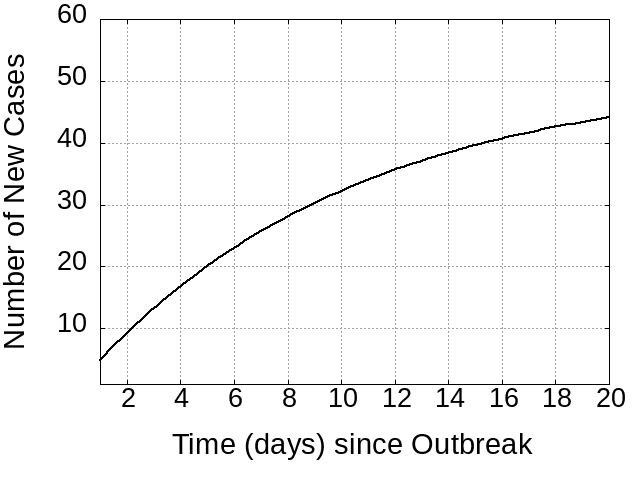
\includegraphics[width=0.45\textwidth]{figures/outbreak.png}
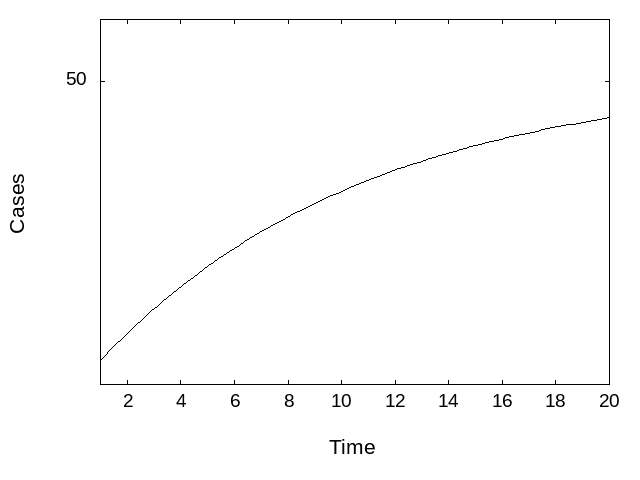
\includegraphics[width=0.45\textwidth]{figures/outbreak2.png}
\caption{\label{fig:outbreak} (Left) One example of a figure describing a viral outbreak. (Right) A different example of the same figure.}
\end{figure}
What differences between the two figures do you notice?  There are several.
\end{frame}

\begin{frame}{Creating Figures and Tables}
Become sharp in \textit{at least one} of these sorts of programs:
\begin{itemize}
\item Excel
\item gnuplot
\item MATLAB/octave
\item python: matplotlib and pyplot
\item Tableau
\item ...
\end{itemize}
\alert{Wardman Library MADLAB and DigLibArts Collaboratory} are there to help you learn.
\end{frame}

\begin{frame}{Creating Figures and Tables}
\small
\begin{figure}
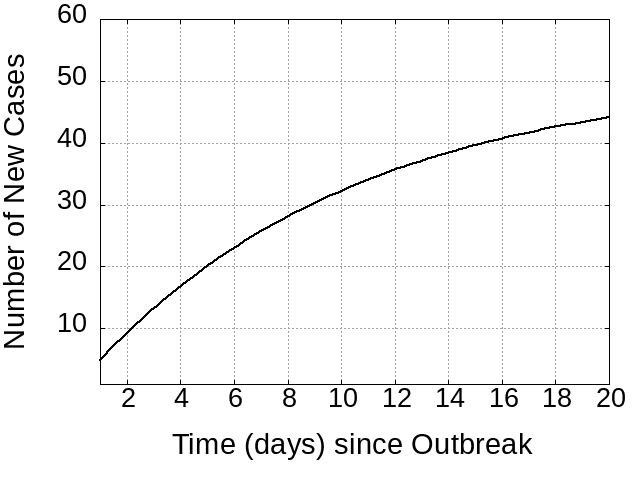
\includegraphics[width=0.4\textwidth]{figures/outbreak.png}
\caption{\label{fig:outbreak2} \textbf{This is the caption.  What belongs here?}}
\end{figure}
\begin{itemize}
\item Yes: Descriptive language: spatial (mostly) and temporal
\item Yes: Guiding the reader through the figure in a logical way (colors, legend, axes, ...)
\item No: Do not provide analysis, opinions, or conclusions in the caption.
\item No: Do not write a long caption.
\end{itemize}
\end{frame}

\begin{frame}{Creating Figures and Tables}
\small
\begin{figure}
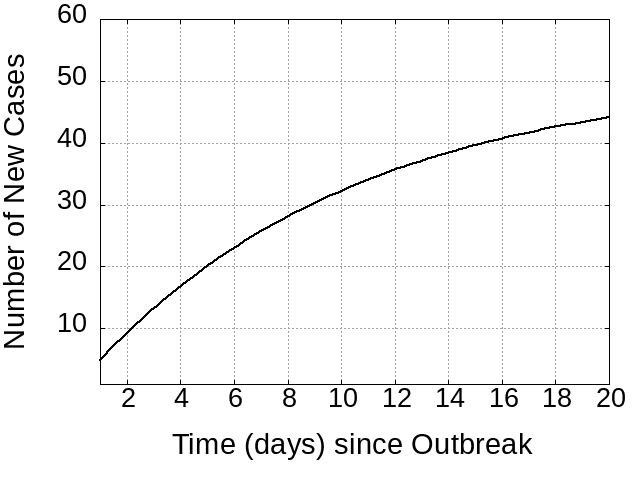
\includegraphics[width=0.4\textwidth]{figures/outbreak.png}
\caption{\label{fig:outbreak3} \textbf{This is the caption.  What belongs here?}}
\end{figure}
\begin{itemize}
\item Yes: Descriptive language: spatial (mostly) and temporal
\item Yes: Guiding the reader through the figure in a logical way (colors, legend, axes, ...)
\item No: Do not provide analysis, opinions, or conclusions in the caption.
\item No: Do not write a long caption.
\end{itemize}
\end{frame}

\begin{frame}{Creating Figures and Tables}
\small
\begin{figure}
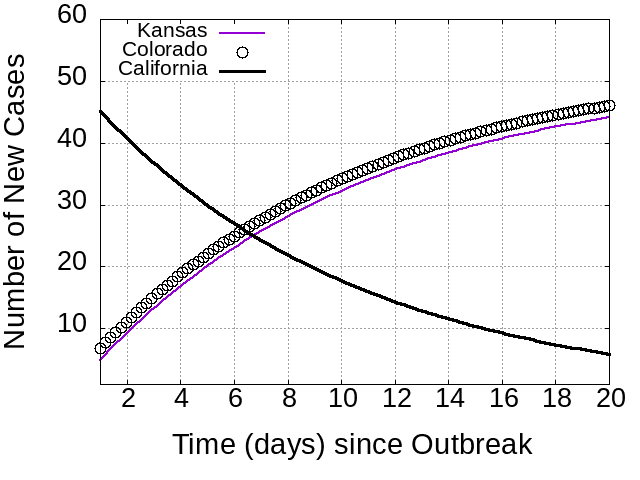
\includegraphics[width=0.5\textwidth]{figures/outbreak3.png}
\caption{\label{fig:outbreak4} The number of new cases per day, versus time in days since the first reported case.  The solid black line corresponds to the State of California, the black circles correspond to the State of Colorado, and the pink line corresponds to the State of Kansas.}
\end{figure}
\end{frame}

\begin{frame}{Creating Figures and Tables}
\small
\begin{figure}
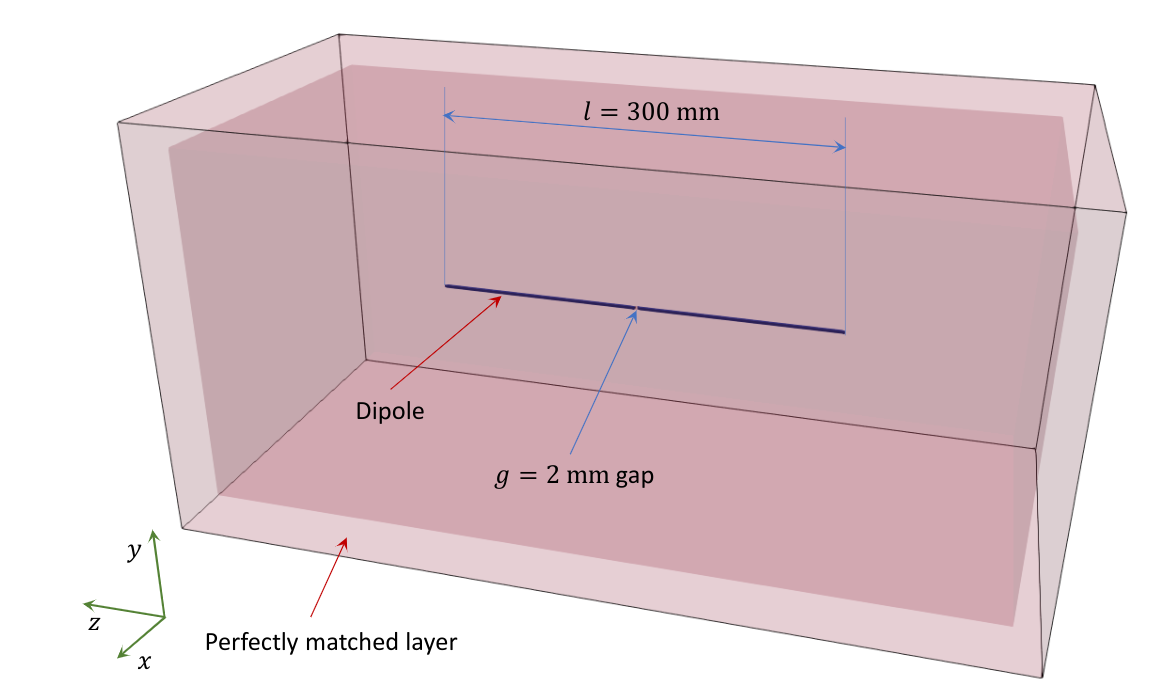
\includegraphics[width=0.75\textwidth]{figures/dipole.png}
\caption{\label{fig:outbreak5} Write the caption that should go here.}
\end{figure}
\end{frame}

\begin{frame}[fragile]{Creating Figures and Tables}
\small
Example code in gnuplot to create the first outbreak figure:
\begin{verbatim}
set key box off
set lmargin 10
set bmargin 5
set xtics font "Arial,20"
set ytics font "Arial,20"
set xlabel "Time (days) since Outbreak" font "Arial,22" offset 0,-1
set ylabel "Number of New Cases" font "Arial,22" offset -2,0
set xrange [1:20]
set yrange [1:60]
set grid
\end{verbatim}
\end{frame}

\begin{frame}[fragile]{Creating Figures and Tables}
\small
Example code in gnuplot to create the first outbreak figure:
\begin{verbatim}
a = 51
b = 0.1
f(x) = a*(1-exp(-b*x))
set terminal png
set output "outbreak.png"
plot f(x) w l lc -1 lw 2
\end{verbatim}
\end{frame}

\section{Conclusion}

\begin{frame}{Conclusion}
\small
\textbf{Week 5}: \textit{The Laboratory Report I:} We will learn the major components of lab reports.  Abstracts, sections and subsections, figures, tables, captions, and how to make them flow and keep the thread of logic intact.
\begin{enumerate}
\item Exercises: how to include a graphic, figure, or table into your writing, and write about it correctly
\item Exercises: how to write an abstract correctly
\item Exercises: how to organize a report into sections and sub-sections
\item Homework: use the map technique to create sections and subsections
\item Homework: trade tracts of writing with someone, and see if they can understand your passive voice style
\end{enumerate}
\end{frame}

\end{document}
